\documentclass[12pt,twocolumn]{article}
\usepackage{graphicx}
\usepackage{pdfpages}
\usepackage{hyperref}
\usepackage[margin=1.25in]{geometry}
\usepackage[utf8]{inputenc}
\graphicspath{ {./Figures/} }
\hypersetup{
    colorlinks=true,
    linkcolor=blue,
    filecolor=magenta,      
    urlcolor=cyan,
}
\urlstyle{same}
\usepackage[font={small,it}]{caption}
\usepackage{fancyvrb}
\title{Model \& Simulation of South Bend Government Call Center using Arena}
\author{John D. Bulger, Jacob D. White \& Adali J.J. Johnson\\Valparaiso University\thanks{``We have neither given or received, nor have we tolerated others' use of unauthorized aid."}}
\date{October 25, 2018}

	\begin{document}
\maketitle

\section{Introduction}
The city of South Bend, located in northern Indiana, established a citizen-accessible call center in February 2013.  It addresses almost every aspect of city-citizen interaction, including waste pick-up and removal, water billing and disconnections, and code enforcement.  By serving as a central hub for communication, the call center is able to consolidate a substantial amount of data regarding citizens as consumers.  This data is available on South Bend's open data portal at \textit{https://data-southbend.opendata.arcgis.com}.

	\begin{figure}[h]
	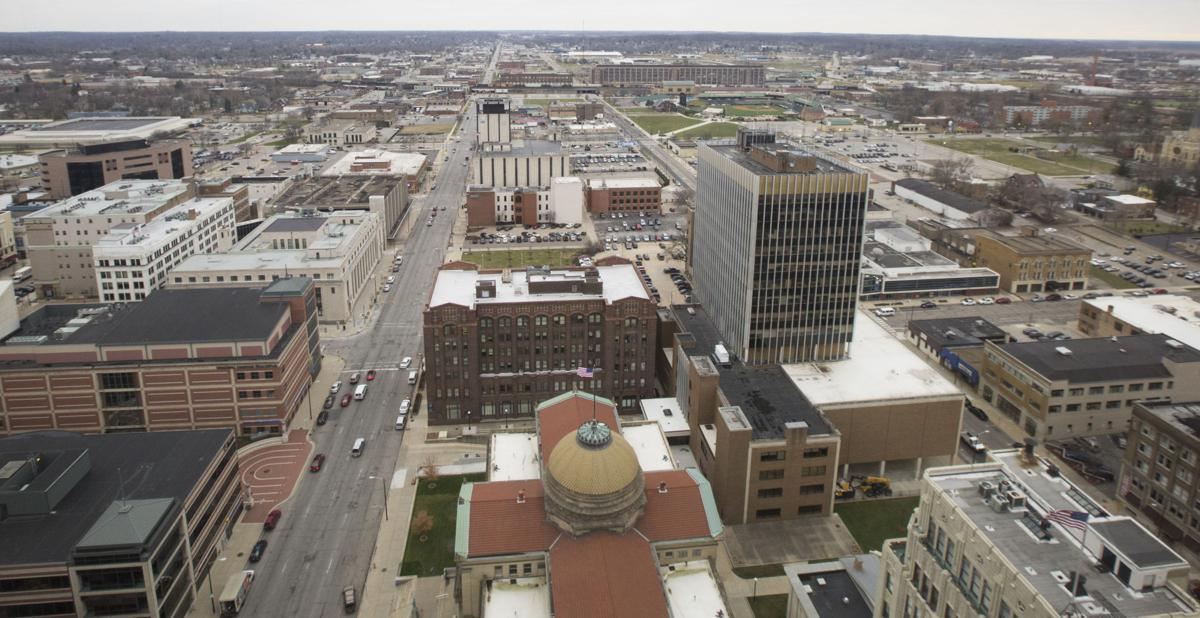
\includegraphics[scale=.17]{south_bend.png}
	\caption{South Bend, IN (Greg Swiercz)}
	\end{figure}

\par
The city's call center is seeking to explore operational efficiency with regard to operator staff.  As such, this model and simulation will be constructed with the primary purpose of discovering the optimal number of agents while maintaining adequate customer satisfaction (measured by time in queue).  Additionally, the model will be modified to explore the addition of a self-service touch-tone option that would allow for callers to complete simple tasks, such as scheduling an extra trash pickup, without speaking to an agent.  Through simulation, these questions were be explored and solved.  The open-source data was processed in Python in order to extract relevant distributions, and the call center was modeled in Arena as a discrete-event model.  

\section{Background}
Call centers are a frequently studied topic within the simulation and modeling disciplines.  As such, some basic terminology shall be explained.  This model consists of two primary components:  calls and operators.  Calls will be represented as entities in Arena, as they are created and move through the system.  For this exploration, an ``arrival" is defined as a unique call first coming into the call process model.  The operators, also known as ``311 liasons," will be represented as resources in Arena.

	\subsection{Prior Work}

Call centers are a prime opportunity to utilize simulation techniques.  In fact, according to Bapat and Pruitte, simulation is the preferred method to analyze and determine the effectiveness of a call center.\cite{bapat}  It allows for evaluation of metrics beyond what a basic analysis encompasses.  For example, the scheduling of call agents should be optimized against call duration and abandonment, as documented by Saltzman and Mehrota.\cite{saltzman}  Such simulations can easily be created to illustrate feasibility of goal accomplishment for corporations while enabling efficient and accurate decision-making.\cite{saltzmeh}

\par


Call center and queuing analysis has been the focus of academic research for years.  Brown et al. provide an excellent overview of the Poisson distribution modeling customer arrivals, as well as the accompanying assumptions.  While arrival distribution is analyzed directly from the data in this model, it will still be implemented as an hourly Poisson distribution. In order to implement this arrival methodology, the authors maintain assumptions that the customers and operators are statistically identical and that they all act independently.\cite{brown}  Zhang, Hong, and Zhang also describe the arrival process as a Poisson distribution, but discuss models which may be more accurate alternatives.\cite{zhang}  They maintain some of the main assumptions as Brown.  Additionally, they point out that differences in time-dependent parameters, customer attitudes and preferences, and operator skill levels should treated as negligible.


\section{Mathematical Model}

Our core model structure is based off the work of Mandelbaun in 2001.  In his frequently referenced text, Mandelbaun lays out the basic schematic of a call center model.  His model illustrates the possible flow of a call starting with its arrival until disposal, be that as a lost call or having completed successfully.\cite{mandelbaun}  While simplistic by nature, the model covers all of the basic aspects of a call center in a sensible format that can easily by applied in Arena.  This model can be seen in Figure 2.  

	\begin{figure}[h]
	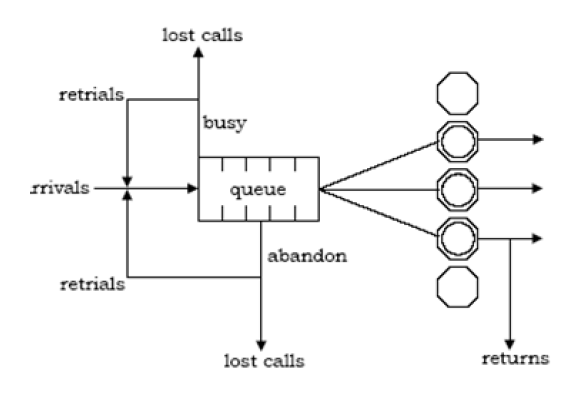
\includegraphics[scale=.45]{call_center_layout.png}
	\caption{Basic Operational Schematic of Call Center (Mandelbaun 2001)}
	\end{figure}

Mandelbaun's model identifies one avenue for arrivals (incoming calls) and three methods of disposal(lost calls due to busy signal, lost calls due to wait time, and completed calls).  Additionally, completed calls have the option to ''return", where they would immediately re-enter the system for whatever reason (perhaps an unresolved issue).  There is a centralized queue before the calls are distributed among resources (operators).  At its core, this is a condensed high-level view of a call center model, specifically designed so that it could easily by expanded as needed for specific analysis.

\subsection{Expanded Model}

The model used for this analysis expands a great deal on the core model identified by Mandelbaun.  In addition to arriving calls, voicemails are ``created" as soon as each simulation ''day" begins, so that the call center has all day to return those calls.  Additionally, some calls get routed to a supervisor after speaking with an agent.  This supervisor resource can then resolve the call, or pass it back to an agent.  This was added in an attempt to model actual call center behavior, where some callers may need assistance beyond a basic agent.  As calls and voicemails arrive and flow through the model, they are assigned three key attributes: topic, language, and priority.


\paragraph{Topic}

Calls are assigned a topic based on the distribution of topics in historical call center data.  In an effort to preserve the simplicity of the model while still utilizing past data, the top six departments (by total number of calls) are specified, with the remaining calls grouped into an ''other" category.  By assigning a topic, the simulation will be able to utilize the historical means and standard deviations of those topics' call durations in order to most accurately replicate the call center.  The departments specifically included in the model account for 90\% of the total call volumes, while the ``other" category constitutes the remaining 10\%.


\paragraph{Language}

Each call and voicemail is assigned a language of either Spanish or English.  The actual call center deals in both of those language, and it has Spanish-speaking operators available.  In order to reflect this, the model's resources all speak English, with some able to speak Spanish as well.  Therefore, arrivals will be routed into two queues:  one for English, and one for Spanish.

\paragraph{Priority}

All incoming calls are assigned a medium priority by default, and voicemails are given the lowest priority (as they can be answered and returned as time permits).  After speaking to an agent, calls needing escalation to a supervisor are given the highest priority (in the event they need to cycle back through the queue again).


\section{Verification \& Validation}

	\subsection{Verification Techniques}
	
	
	\subsection{Validation Plan}
	
	
\section{Simulation}

	\subsection{Base Simulation Setup}
This simulation utilizes an accurate representation of arrivals as calculated from the aforementioned open-source data.  Mean call arrivals were identified down to the hour for each weekday.  The results allows for the arrivals to be scheduled as such in Arena.  This will base the actual volume of calls in line with prior historical trends, as opposed to applying a rough blanket estimate.  The scheduling of operators (resources) is also dictated by historical data.  The operator schedule was supplied by call center management.  This schedule can be seen in Figure 3.  

	\begin{figure}[h]
	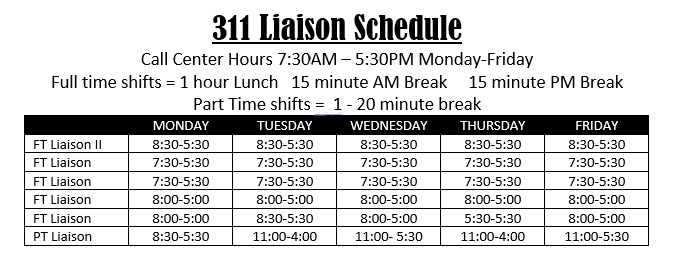
\includegraphics[scale=.35]{schedule2.jpg}
	\caption{Call center operator schedule}
	\end{figure}

\section{Results}

\section{Discussion}


\section{Conclusion}

	\subsection{Challenges}

	\subsection{Opportunities for Further Study}














\newpage
\clearpage
\pagenumbering{gobble}
\begin{thebibliography}{7}
	
	\bibitem{bapat}
	Bapat, V. \& Pruitte, E.B. Jr.. (1998). Using simulation in call centers. \textit{In Proceedings of the 30th conference on Winter simulation (WSC '98)}, D. J. Medeiros, Edward F. Watson, John S. Carson, and Mani S. Manivannan (Eds.). IEEE Computer Society Press, Los Alamitos, CA, USA, 1395-1400.
	
	\bibitem{saltzman}
	Saltzman, R.M. \& Mehrotra, V.. (2007). Managing trade-offs in call center agent scheduling: methodology and case study. \textit{In Proceedings of the 2007 Summer Computer Simulation Conference (SCSC '07)}. Society for Computer Simulation International, San Diego, CA, USA, 643-651.
	
	\bibitem{saltzmeh}
	Saltzman, R.M. \& Mehrota, V. (2001). A call center uses simulation to drive strategic change. \textit{Interfaces 31}(3). \href{https://doi.org/10.1287/inte.31.3.87.9632}{https://doi.org/10.1287/inte.31.3.87.9632}. 
	
	
	\bibitem{baraka}
	Baraka, H., Baraka H. \& El-Gamily, I. (2013). Assessing call centers' success: A validation of the DeLone and Mclean model for information system. \textit{Egyptian Informatics Journal, 14}, 99-108.

	\bibitem{brown}
	Brown, L., Gans, N., Mandelbaum, A., Sakov, A., Shen, H., Zeltyn, S., \& Zhao, L. (2005). Statistical analysis of a telephone call center: a queueing-science perspective. \textit{Journal of the American Statistical Association, 100}(469), 36-50.

	\bibitem{zhang}
	Zhang X., Jeff Hong L., \& Zhang J.. (2014). Scaling and modeling of call center arrivals. \textit{In Proceedings of the 2014 Winter Simulation Conference (WSC '14)}. IEEE Press, Piscataway, NJ, USA, 476-485.

	\bibitem{mandelbaun}
	Mandelbaun A., Sakov A., \& Zeltyn S.. (2001). Empirical Analysis of a Call Center. Technion Israel Institute of Technology, Israel.

\end{thebibliography}

\end{document}